\documentclass[11pt,a4paper,DIV=10,]{scrartcl}
%\usepackage[latin1]{inputenc}
\usepackage[utf8]{inputenc}
\usepackage{lmodern}
\usepackage[ngerman]{babel}
\usepackage{amsmath}
\usepackage{amsfonts}
\usepackage{amssymb}
\usepackage{fancybox}
\usepackage{multicol}
\usepackage{graphicx}
\usepackage{color}
\usepackage{colortbl}
% Define user colors using the RGB model
\definecolor{dunkelgrau}{rgb}{0.8,0.8,0.8}
\definecolor{hellgrau}{rgb}{0.95,0.95,0.95}
\usepackage{booktabs}
\usepackage[normal,font={small,color=black}, labelfont=bf,figurename=Abb.]{caption}
\usepackage{float}
\usepackage{cite}
\usepackage{url}
\bibliographystyle{unsrtnat}
\usepackage[numbers]{natbib}
\usepackage[T1]{fontenc}

\begin{document}
\onecolumn
\subsection*{Versuchsprotokoll zum 1. Kurstag }
\section*{Zum Wasserhaushalt von Pflanzen\\Bestimmung des Wasserpotenzials bei \textit{Solanum Tuberosum}}
\textbf{Christoph van Heteren-Frese\footnotemark[1], Jana Jerosch\footnotemark[1], Nora Pauli\footnotemark[1]} \\[0.1cm]
\footnotemark[1]Freie Universität Berlin\\[0.2cm]
Eingereicht am 13.11.2012\\
\hrule

\section*{Einleitung}    
%Das vorliegende Protokoll wurde von den Autoren im Rahmen des pflanzenphysiologischen Grundpraktikums als Bestandteil des Moduls \textit{Physiologie und Biochemie der Pflanzen und Tiere} der Freien Universität Berlin verfasst. 
Zellen müssen ihren Wasserhaushalt regulieren um lebensfähig zu bleiben. Der dafür notwendige Wasseraustausch erfolgt durch \textbf{Osmose}, bei der Wasser durch eine semipermeable Membran\footnote{Die Membran ist für die gelösten Stoffe undruchlässig.}  entlang eines chemischen Gradienten fließt; von der Lösung mit der niedrigeren Stoffkonzentration in die Lösung mit der höheren Stoffkonzentration. Dieses Prinzip bildet die Grundlage für den vorliegenden Versuch, bei dem das Wasserpotenzial von \textit{Solanum Tuberosum} bestimmt wurde. 

\subsection*{Wasserpotential}

Als Wasserpotential\footnote{Der Wortteil \textit{potential} bezieht sich auf die potentielle Energie des Wassers, also seine Fähigkeit Arbeit zu verrichten. Dies kann z.B. zur Ausdehnung der Zelle führen.} bezeichnet man die Kapazität einer Zelle Wasser durch Osmose
aufzunehmen. Die hierfür verwendete Einheit ist der Druck (Pascal). Das Wasserpoten-
zial ist somit eine Kenngröße, durch die der Wassergehalt von Zellen charakterisiert
werden kann. Dabei ist das Wasserpotential $\Psi$ definiert als das chemische Potential des
Wassers in Bezug zu einen Grundzusdstand (reines Wasser) pro Molvolumen. Grund-
sätzlich bewegt sich freies Wasser vom Ort des höheren Wasserpotenzials zum Ort des
niedrigeren Wasserpotenzials. Ist das Wasserpotenzial an beiden Orten gleich, findet
\textbf{kein} Wasserfluss statt.

%Das Wasserpotenzial ist eine Kenngröße, mit dem der Wassergehalt von Zellen charakterisiert werden kann. Dabei ist das Wasserpotential $\Psi$ definiert als das chemische Potential des Wassers in Bezug zu einen Grundzusdstand (reines Wasser) pro Molvolumen. Grundsätzlich bewegt sich freies Wasser vom Ort des höheren Wasserpotenzials zum Ort des niedrigeren Wasserpotenzials. Ist das Wasserpotenzial an beiden Orten gleich, findet \textbf{kein} Wasserfluss statt.
\section*{Material und Methoden}
\begin{enumerate}
	\item[•] 1 Kartoffel (\textit{Solanum Tuberosum})
	\item[•] Saccharose-Stammlösung (1 Mol)
\end{enumerate}
\subsection*{Durchführung}
Aus der Saccharose-Stammlösung wurde eine Verdünnungsreihe erstellt und in fünf Petrischalen gegeben (Konzentrationen siehe Tabelle \ref{tab1}). Ein Teil der Kartoffel wurde in Würfel von ca. $5\times5\times5$ mm Kantenlänge geschnitten und anschließend in Portionen von jeweils ca. fünf Gramm in die unterschiedlich konzentrierte Sacharose-Lösung gegeben. Nach drei Stunden wurden die Gewebeproben aus der Lösung genommen und gewogen.
\section*{Ergebnisse}
Die Ergbnisse sind in Tabelle 1 und Abbildung 1 dargestellt.
\begin{table}[H]
\caption{Masse von fünf Gewebeproben von \textit{Solanum Tuberosum} vor und nach einem dreistündigen Bad in Saccharose-Lösung .}
\label{tab1}
\center
\begin{tabular}{cccc}
\toprule
Konzentrtion &\multicolumn{2}{c}{Gewicht in g} & Zu- bzw. Abnahme \\
in Mol &vorher & nacher & in \%\\
\midrule
0,20 & 5,050 & 5,257 & 4,10 \\
0,25 & 5,035 & 4,947 & -1,95\\
0,30 & 5,080 & 4,867 & -4,19\\
0,35 & 5,078 & 4,295 & -15,42\\
0,40 & 5,076 & 4,539 & -10,58\\
\bottomrule
\end{tabular}
\end{table}
% Hier beginnt das erste Bild 
\begin{figure}[H]
\center
\captionsetup{width=1\textwidth}	
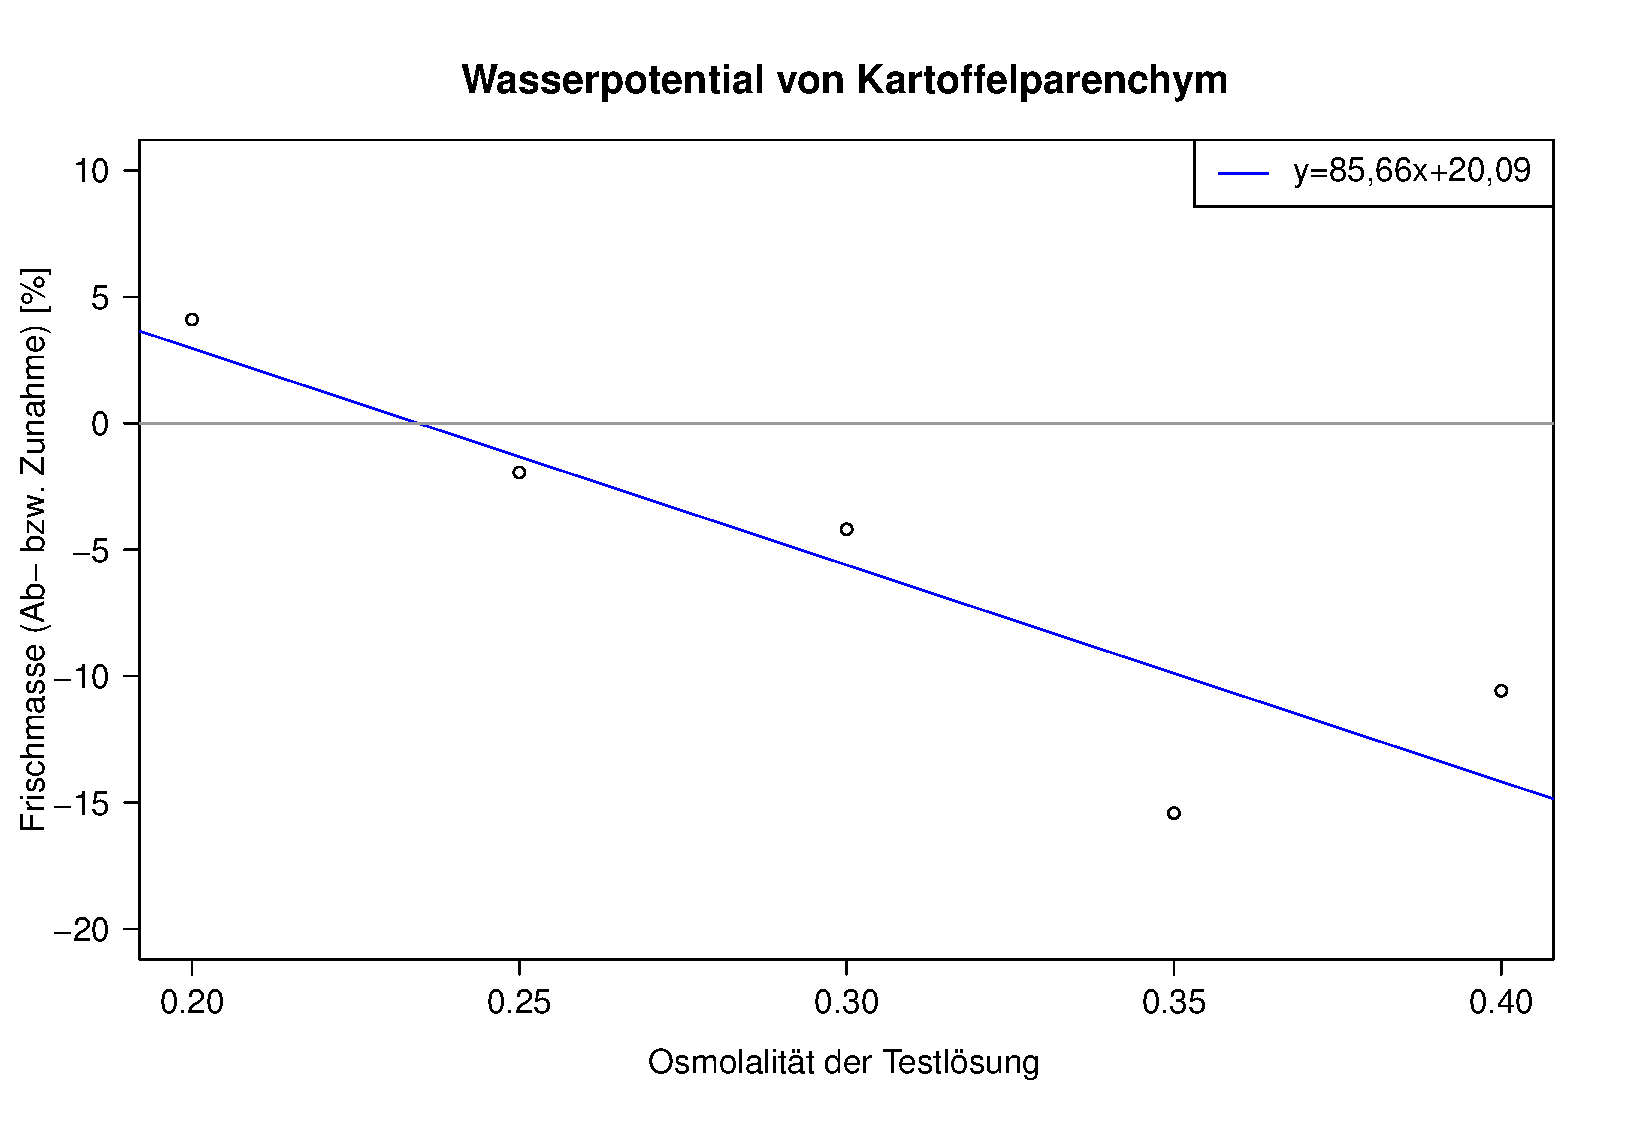
\includegraphics[width=1.0\textwidth]{Abbildungen/Rplot01}
\caption{Abhhängigkeit der Ab- bzw. Zunahme der Masse von der Osmolalität von \textit{Solanum Tuberosum}. Die Regressionsgerade zeigt eine deutliche Tendenz.}
\label{v1}
\end{figure}
\noindent
Mit Hilfe einer Regressionsgerade, die durch die Gleichung
\begin{equation}
y= -85,66x+20,09
\end{equation}
beschrieben wird, kann die Konzentration, bei der keine Ab- bzw. Zunahme der Masse stattfindet, berechnet werden. Durch umstellen von (1) ergibt sich ein Wert von
\begin{equation}
x=0,23 \textrm{~Mol}
\end{equation}
Mit der Gleichung
\begin{equation}
\Psi_W=-c\cdot R\cdot T
\end{equation}
kann das Wasserpotential $\Psi_W$ für $x=c$ berechnet werden:
\begin{equation}
\Psi_W=-0,23 \textrm{~Mol} \cdot 8,314 \textrm{~J}\cdot\textrm{K}^{-1}\cdot \textrm{mol}^{-1}\cdot 295 K=0,56 \textrm{~MPa}
 \end{equation}
\section*{Diskussion}
Die erhaltenen Ergebnisse entsprechen den Erwartungen und werden durch die gängige Literatur abgedekt. Die ermittelte Regressionsgerade zeigt eine lineare Abnahme, die theoretisch so zu erwarten gewesen ist. 

Wird pflanzliches Gewebe in eine Lösung getaucht, derren Wasserpotenzial \textit{höher} als das der Zellen in dem Gewebe ist, fließt Wasser in diese Zellen hinein. Somit nimmt die Masse des Gewebes zu. Wird das Gewebe in eine Lösung gegeben, derren Wasserpotential \textit{niedriger} als das des Gewebes ist, fließt Wassser aus den Zellen heraus und die Masse nimmt ab. Abbildung \ref{v1} veranschaulicht dieses Phänomen. 

Fehler könnten beim Ansetzen der Verdünnungsreihe enstanden sein. Des Weiteren sind die
Messungenauigkeiten der verwendeteten Pipetten zu berücksichtigen. 
\end{document}